%%%%%%%%%%%%%%%%%%%%%%%%%%%%%%%%%%%%%%%%
% Beamer Presentation
% LaTeX Template
% Version 1.0 (10/11/12)
%
% This template has been downloaded from:
% http://www.LaTeXTemplates.com
%
% License:
% CC BY-NC-SA 3.0 (http://creativecommons.org/licenses/by-nc-sa/3.0/)
%
%%%%%%%%%%%%%%%%%%%%%%%%%%%%%%%%%%%%%%%%%

%----------------------------------------------------------------------------------------
%	PACKAGES AND THEMES
%----------------------------------------------------------------------------------------

\documentclass[xcolor=dvipsnames, aspectratio=169]{beamer}

\mode<presentation> {

% The Beamer class comes with a number of default slide themes
% which change the colors and layouts of slides. Below this is a list
% of all the themes, uncomment each in turn to see what they look like.

\usetheme{Madrid} %Hannover
% As well as themes, the Beamer class has a number of color themes
% for any slide theme. Uncomment each of these in turn to see how it
% changes the colors of your current slide theme.
\useoutertheme{infolines} % Alternatively: miniframes, infolines, split
\useinnertheme{circles}
\definecolor{UBCblue}{rgb}{0.04706, 0.13725, 0.26667} % UBC Blue (primary)
\usecolortheme[named=UBCblue]{structure}
}

\usepackage{graphicx} % Allows including images
\usepackage{booktabs} % Allows the use of \toprule, \midrule and \bottomrule in tables
\usepackage{textpos}
\usepackage{caption}
\usepackage[utf8]{inputenc}
\usepackage[brazilian]{babel}
\usepackage{csquotes}
\usepackage{listings}
\setbeamertemplate{caption}[numbered]
\usepackage[style=abnt]{biblatex}
\addbibresource{bibliography.bib}
\PassOptionsToPackage{useregional}{datetime2}
\usepackage{xcolor}


\definecolor{codegreen}{rgb}{0,0.6,0}
\definecolor{codegray}{rgb}{0.5,0.5,0.5}
\definecolor{codepurple}{rgb}{0.58,0,0.82}
\definecolor{backcolour}{rgb}{0.95,0.95,0.92}
\definecolor{string-color}{rgb}{0.3333, 0.5254, 0.345}

\lstdefinestyle{mystyle}{
    backgroundcolor=\color{backcolour},   
    commentstyle=\color{codegreen},
    keywordstyle=\color{string-color},
    keywordstyle=[2]{\color{codepurple}},
    keywordstyle=[3]{\color{magenta}},
    numberstyle=\tiny\color{codegray},
    stringstyle=\color{codepurple},
    basicstyle=\ttfamily\footnotesize,
    breakatwhitespace=false,         
    breaklines=true,                 
    captionpos=b,                    
    keepspaces=true,                 
    numbers=left,                    
    numbersep=5pt,                  
    showspaces=false,                
    showstringspaces=false,
    showtabs=false,                  
    tabsize=2,
    otherkeywords = {tf, Sequential, SimpleRNN, Dense, GRU, LSTM},
    morekeywords = [3]{keras},
}

\lstset{style=mystyle}
\newcommand{\source}[1]{\vspace{-20pt} \caption*{ Fonte: {#1}} }
\usepackage{copyrightbox}


\makeatletter
% \beamer@nav@subsectionstyle{hide/hide/hide}
\addtobeamertemplate{sidebar left}{%
\hspace{0.5cm}
\includegraphics[width=0.9cm, keepaspectratio]{figures/_brasao_ufsm_cor.png}
% \hspace{2.3cm}
\includegraphics[width=0.8cm, keepaspectratio]{figures/brasao_ctism.png}
% \hspace{2.3cm}\includegraphics[width=1.5cm, keepaspectratio]{_logosbc.png}
% \hspace{2.3cm}\includegraphics[width=1.5cm, keepaspectratio]{_logoERRC.png}%
}{}


\setbeamertemplate{footline}
{
	\leavevmode%
	\hbox{%
	    % \hspace{0.5cm}
\includegraphics[width=0.8cm, keepaspectratio]{figures/_brasao_ufsm_cor.png}
		\begin{beamercolorbox}[wd=.333333\paperwidth,ht=2.25ex,dp=1ex,right]{date in head/foot}%
			\usebeamerfont{date in head/foot}\insertshortdate{}\hspace*{2em}
			\insertframenumber{} / \inserttotalframenumber\hspace*{2ex} 
		\end{beamercolorbox}}%
		%\vskip0pt%
	}
\makeatother

%----------------------------------------------------------------------------------------
%	TITLE PAGE
%----------------------------------------------------------------------------------------

\title[INTERNAL POSITION ERROR CORRECTION]{INTERNAL POSITION ERROR CORRECTION} % The short title appears at the bottom of every slide, the full title is only on the title page

\author[FDR]{Fábio Demo da Rosa} % Your name
%\includegraphics[]{logositeredes.png}
\institute[UFSM] % Your institution as it will appear on the bottom of every slide, may be shorthand to save space
{
Universidade Federal de Santa Maria \\ % Your institution for the title page
Pós-Graduação em Ciência da Computação \\
Disciplina de Robótica Móvel\\
\medskip
\textit{faberdemo@gmail.com} % Your email address
}
\date{\today} % Date, can be changed to a custom date
\newcounter{saveenumi}
\newcommand{\seti}{\setcounter{saveenumi}{\value{enumi}}}
\newcommand{\conti}{\setcounter{enumi}{\value{saveenumi}}}

\resetcounteronoverlays{saveenumi}


\begin{document}

\begin{frame}
\titlepage % Print the title page as the first slide
\end{frame}

\begin{frame}
\frametitle{Visão Geral} %\includegraphics[]{logositeredes.png}} % Table of contents slide, comment this block out to remove it
\tableofcontents % Throughout your presentation, if you choose to use \section{} and \subsection{} commands, these will automatically be printed on this slide as an overview of your presentation
\end{frame}

%----------------------------------------------------------------------------------------
%	PRESENTATION SLIDES
%----------------------------------------------------------------------------------------

%------------------------------------------------
\section{Introdução}
%------------------------------------------------
\begin{frame}[allowframebreaks, fragile]
  \frametitle{Introdução}
  \begin{itemize}
    \item INTERNAL POSITION ERROR CORRECTION (IPEC)
    \item Contexto de robôs móveis e desafios de dead-reckoning
      \begin{itemize}
        \item Relevância de robôs em processos de automação industrial ou tarefas repetitivas, elevando a eficiência e precisão;
        \item Dificuldades de navegação dos robôs, como deslizamento das rodas e erros acumulativos na estimativa de posição.
      \end{itemize}
    \item Objetivo do método IPEC
      \begin{itemize}
        \item Como o IPEC visa corrigir erros na estimativa da posição do robô;
        \item Aborda o aprimoramento na estimativa da direção que o robô está apontando.
      \end{itemize}
    \item Apresentação do veículo CLAPPER como caso de estudo
    \newpage
    \begin{figure}
      \centering
      \copyrightbox[b]{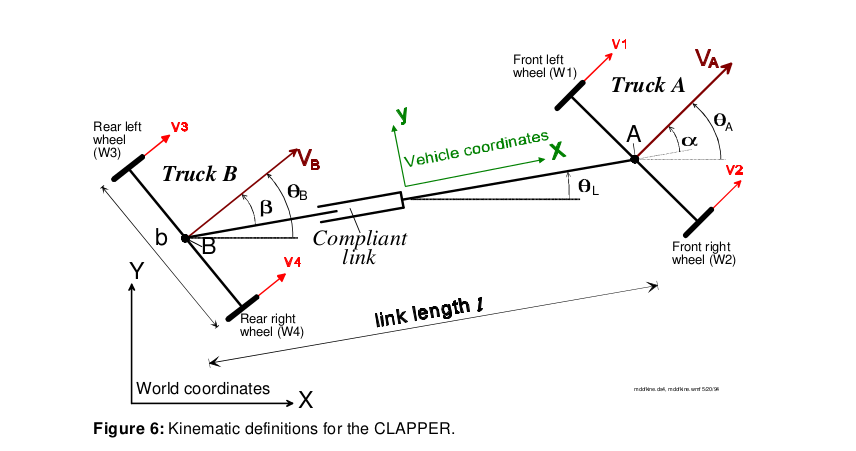
\includegraphics[scale=0.35]{figures/1_Kinematic_definitions_for_the_CLAPPER.png}}%
      {Fonte: \cite{borenstein1995intemal}}
      \caption{O módulo antena/trasmissor/receptor é montado na frente (ou lateral) do veículo}
      \label{fig:curva_de_freq}
    \end{figure} 
  \end{itemize}
\end{frame}

%------------------------------------------------
\section{Metodologia}
%------------------------------------------------
\begin{frame}{Metodologia}
  \begin{itemize}
    \item Sensores ultrassônicos são usados no CLAPPER
      \begin{itemize}
        \item Para detectar objetos evitar colisões.
        \item Medição de distância até um objeto, auxiliando na navegação.
      \end{itemize}
    \item Planejamento de caminho e monitoramento
      \begin{itemize}
        \item Algoritmos responsáveis por traçar a rota que o robô deve seguir.
        \item Como o sistema ajusta o caminho com base nos dados dos sensores e outras informações.
      \end{itemize}
  \end{itemize}
\end{frame}

%------------------------------------------------
\section{Experimentos}
%------------------------------------------------
\begin{frame}{O Experimento da Linha Reta}
  \begin{itemize}
    \item Configurações de testes com e sem IPEC
      \begin{itemize}
        \item A velocidade é um fator nos experimentos.
        \item O tipo de superfície em que o robô se move.
      \end{itemize}
    \item Efeitos de "bumps" na trajetória
      \begin{itemize}
        \item Impacto nas medidas
        \item Correções necessárias
      \end{itemize}
    \item Resultados de erros de posição e orientação
      \begin{itemize}
        \item Comparação estatística
        \item Gráficos de desempenho
      \end{itemize}
  \end{itemize}
\end{frame}

\begin{frame}{O Experimento do Caminho Retangular}
  \begin{itemize}
    \item Desafios em trajetórias fechadas
      \begin{itemize}
        \item Problemas de acumulação de erros
        \item Correções em tempo real
      \end{itemize}
    \item Importância de testar em ambas as direções
      \begin{itemize}
        \item Impacto na simetria da trajetória
        \item Coleta de dados
      \end{itemize}
    \item Resultados e comparação com e sem IPEC
      \begin{itemize}
        \item Métricas de erro
        \item Validade das correções
      \end{itemize}
  \end{itemize}
\end{frame}

%------------------------------------------------
\section{Resultados}
%------------------------------------------------
\begin{frame}{Resultados}
  \begin{itemize}
    \item Melhoria significativa na precisão do dead-reckoning
      \begin{itemize}
        \item Quantificação da melhoria
        \item Implicações práticas
      \end{itemize}
    \item Redução dos erros de orientação
      \begin{itemize}
        \item Impacto no planejamento de caminho
        \item Benefícios a longo prazo
      \end{itemize}
    \item Resultados em diferentes condições de piso
      \begin{itemize}
        \item Variação dos resultados
        \item Escopo de aplicabilidade
      \end{itemize}
  \end{itemize}
\end{frame}

%------------------------------------------------
\section{Aplicações e Trabalho Futuro}
%------------------------------------------------
\begin{frame}{Aplicações e Trabalho Futuro}
  \begin{itemize}
    \item Aplicação em ambientes industriais e agrícolas
      \begin{itemize}
        \item Redução de custos
        \item Aumento da eficiência
      \end{itemize}
    \item Extensão para outros tipos de veículos
      \begin{itemize}
        \item Drones
        \item Veículos aquáticos
      \end{itemize}
    \item Investigação em robôs colaborativos
      \begin{itemize}
        \item Sincronização
        \item Comunicação inter-robô
      \end{itemize}
  \end{itemize}
\end{frame}


%------------------------------------------------
\section{Conclusões}
%------------------------------------------------
\begin{frame}{Conclusões}
  \begin{itemize}
    \item Resumo das contribuições do método IPEC
      \begin{itemize}
        \item Eficácia na correção de erros
        \item Versatilidade de aplicação
      \end{itemize}
    \item Importância da correção imediata dos erros
      \begin{itemize}
        \item Redução do retrabalho
        \item Melhoria na confiabilidade
      \end{itemize}
    \item Validade do método em diferentes cenários
      \begin{itemize}
        \item Extensão do estudo
        \item Limitações encontradas
      \end{itemize}
  \end{itemize}
\end{frame}


%------------------------------------------------
%\section*{Referências}
%------------------------------------------------
\begin{frame}
    % \nocite{*}
    \printbibliography
\end{frame}


\begin{frame}
\titlepage % Print the title page as the first slide
\end{frame}

\end{document}